\documentclass{scrartcl}

\usepackage{german}
\usepackage[utf8]{inputenc}  %Umlaute
\usepackage[T1]{fontenc}     %Umlauttrennung
\usepackage{lmodern}         %modernes Schriftbild
\usepackage{amsmath}         %math Umgebungen
\usepackage{graphicx}
\usepackage{hyperref}        %URLs
\usepackage{gensymb}         %Gradzeichen
\usepackage{float}           %Positionierung von Tabellen und Abb
\usepackage{textgreek}


\begin{document}
\begin{titlepage}
  \begin{center}
    \vspace*{1cm}
    \LARGE
    Physikpraktikum für Naturwissenschaftler \\
    \vspace*{1cm}
    \Huge
    \textbf{Versuch: Kennlinien} \\
    \vspace*{0.3cm}
    \Large
    Durchgeführt am 17. Januar 2019 \\
    Betreuer: Johannes Fendt \\
    \vspace*{2.5cm}
    Gruppe 13 \\
    Felix Burr: felix.burr@uni-ulm.de \\
    Johannes Spindler: johannes.spindler@uni-ulm.de \\
    \vfill 
  \end{center}
  Wir bestätigen hiermit, das Protokoll selbstständig erarbeitet zu haben und in genauer Kenntnis über dessen Inhalt zu sein. \\
  \vspace*{0.8cm}
  \\
  Felix Burr
  \hfill
  Johannes Spindler
\end{titlepage}
\pagebreak
\tableofcontents


\pagebreak

\section{Einleitung}
Die Stromstärke $I$ eines elektrischen Stroms ist definiert als die Ladungsmenge $\Delta Q$, die pro Zeitintervall $\Delta t$ durch einen Querschnitt des Stromkreises fließt:
\begin{align}
I = \frac{\Delta Q}{\Delta t} = \frac{dQ}{dt}
\end{align}
Das bedeutet, der in einem Material fließende Strom bei einer gegebenen Spannung hängt von der Fähigkeit des Materials ab, Ladungen zu transportieren. Diese mikroskopische Eigenschaft wird als elektrische Leitfähigkeit $\sigma$ des Materials bezeichnet. Es besteht folgender Zusammenhang mit makroskopischen Größen:
\begin{align}
\sigma = G \frac{l}{A} = \frac{I}{U} \cdot \frac{l}{A}
\end{align}
Hier bezeichnet $G = \frac{I}{U}$ den Leitwert, $l$ die Leiterlänge und $A$ die Querschnittsfläche. Diese makroskopischen Größen sind leicht messbar.

Das makroskopisch messbare elektrische Verhalten des Stromkreises wird in Form von Kennlinien dargestellt. Dazu wird eine Spannung angelegt, schrittweise variiert und jeweils der Stromfluss gemessen. Die Wertepaare werden in einem $U$-$I$-Diagramm aufgetragen. In diesem Versuch werden so die Bauteile Metallfaden- und Kohlefadenlampe, Halbleiter-Diode und MOS-FET untersucht.




\pagebreak
\section{Kennlinien von Metallfaden- und Kohlefadenlampe}
\subsection{Versuchsaufbau und Durchführung}

\begin{figure}[H]
  \centering
    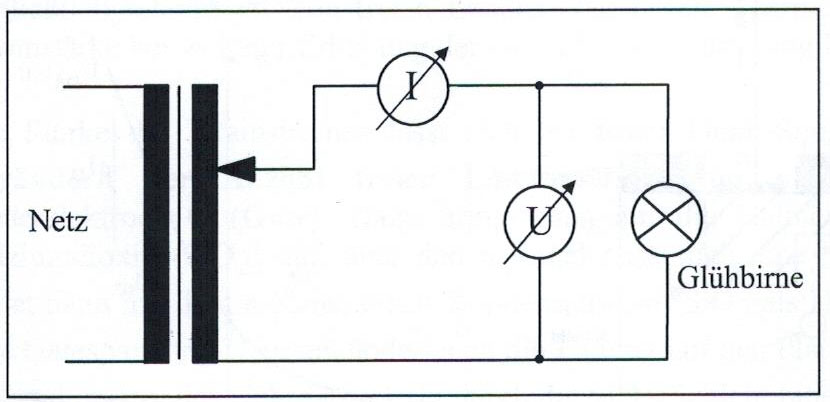
\includegraphics[scale=0.75]{Aufbau1.JPG}
  \caption{Schaltbild zur Messung an einer Lampe (aus der Versuchsanleitung)}
  \label{fig:Aufbau1}
\end{figure}

Wie in Abbildung \ref{fig:Aufbau1} gezeigt, wird die Lampe an ein Netzgerät angeschlossen, mit welchem Spannungen $U$ zwischen -40V und +40V in 2,5V-Schritten angelegt werden (zwischen -5V und +5V aber 1V-Schritte). Mithilfe eines parallel-geschalteten Voltmeters kann die Spannung noch genauer eingestellt werden. Das in Reihe geschaltete Amperemeter dient zur Messung des Stroms $I$.

Anschließend werden für jede Spannung die Verlustleistung $P$ und der Widerstand $R$ berechnet:
\begin{align}
P &= U \cdot I \\
R &= \frac{U}{I}
\end{align}
Für $U = 0V$ muss der Widerstand stattdessen als Inverses der Steigung in der Kennlinie bestimmt werden:
\begin{align}
R(0V) = \frac{1V-(-1V)}{I(1V)-I(-1V)} = \frac{2V}{I(1V)-I(-1V)}
\end{align}
Damit werden die Kennlinie und das $P$-$R$-Diagramm erstellt und diskutiert.

Als Lampe wird zuerst eine Kohlefaden-, dann eine Metallfadenlampe verwendet.
\subsection{Messwerte und Ergebnisse}
\begin{table}[H]
\captionof{table}{Messwerte für I und daraus errechnete Werte für P und R bei schrittweise variierter Spannung U für eine Kohlefadenlampe.}
\begin{center}
\begin{tabular}{l|l|l|l}
U [V]   &   I [mA]   &   P [W]   &   R [\textOmega]\\
\hline
-40,0   &   -24,6   &   0,984   &   1630 \\
-37,5   &   -22,9   &   0,859   &   1640 \\
-35,0   &   -21,1   &   0,739   &   1660 \\
-32,5   &   -19,5   &   0,634   &   1670 \\
-30,0   &   -17,9   &   0,537   &   1680 \\
-27,5   &   -16,2   &   0,446   &   1700 \\
-25,0   &   -14,6   &   0,365   &   1710 \\
-22,5   &   -13,1   &   0,295   &   1720 \\
-20,0   &   -11,5   &   0,230   &   1740 \\
-17,5   &   -9,9    &   0,173   &   1770 \\
-15,0   &   -8,4    &   0,126   &   1790 \\
-12,5   &   -7,0    &   0,087   &   1790 \\
-10,0   &   -5,5    &   0,055   &   1820 \\
-7,5    &   -4,0    &   0,030   &   1880 \\
-5,0    &   -2,6    &   0,013   &   1920 \\
-4,0    &   -2,1    &   0,0084  &   1900 \\
-3,0    &   -1,6    &   0,0048  &   1880 \\
-2,0    &   -1,0    &   0,0020  &   2000 \\
-1,0    &   -0,5    &   0,0005  &   2000 \\
0       &   0       &   0       &   2000 \\
+1,0    &   +0,5    &   0,0005  &   2000 \\
+2,0    &   +1,0    &   0,0020  &   2000 \\
+3,0    &   +1,6    &   0,0048  &   1880 \\
+4,0    &   +2,2    &   0,0088  &   1820 \\
+5,0    &   +2,7    &   0,014   &   1850 \\
+7,5    &   +4,1    &   0,031   &   1830 \\
+10,0   &   +5,5    &   0,055   &   1820 \\
+12,5   &   +7,0    &   0,088   &   1790 \\
+15,0   &   +8,5    &   0,128   &   1760 \\
+17,5   &   +10,0   &   0,175   &   1750 \\
+20,0   &   +11,5   &   0,230   &   1740 \\
+22,5   &   +13,0   &   0,293   &   1730 \\
+25,0   &   +14,6   &   0,365   &   1710 \\
+27,5   &   +16,2   &   0,446   &   1700 \\
+30,0   &   +17,8   &   0,534   &   1690 \\
+32,5   &   +19,5   &   0,634   &   1670 \\
+35,0   &   +21,1   &   0,739   &   1660 \\
+37,5   &   +22,8   &   0,855   &   1640 \\
+40,0   &   +24,5   &   0,980   &   1630 
\end{tabular}
\end{center}
\label{tab:Kohlefadenlampe}
\end{table}

\begin{table}[H]
\captionof{table}{Messwerte für $I$ und daraus errechnete Werte für $P$ und $R$ bei schrittweise variierter Spannung $U$ für eine Metallfadenlampe.}
\begin{center}
\begin{tabular}{l|l|l|l}
U [V]   &   I [mA]   &   P [W]   &   R [\textOmega]\\
\hline
-40,0   &   -24,5   &   0,980   &   1630 \\
-37,5   &   -23,5   &   0,881   &   1600 \\
-35,0   &   -22,5   &   0,788   &   1560 \\
-32,5   &   -21,5   &   0,699   &   1510 \\
-30,0   &   -20,5   &   0,615   &   1460 \\
-27,5   &   -19,3   &   0,531   &   1420 \\
-25,0   &   -18,3   &   0,458   &   1370 \\
-22,5   &   -17,1   &   0,385   &   1320 \\
-20,0   &   -15,9   &   0,318   &   1260 \\
-17,5   &   -14,6   &   0,256   &   1200 \\
-15,0   &   -13,3   &   0,200   &   1130 \\
-12,5   &   -11,8   &   0,148   &   1060 \\
-10,0   &   -10,3   &   0,103   &    970 \\
-7,5    &   -8,6    &   0,065   &    870 \\
-5,0    &   -6,7    &   0,034   &    750 \\
-4,0    &   -6,2    &   0,025   &    650 \\
-3,0    &   -5,3    &   0,016   &    570 \\
-2,0    &   -4,2    &   0,0084  &    480 \\
-1,0    &   -2,4    &   0,0024  &    420 \\
0       &   0       &   0       &    410 \\
+1,0    &   +2,5    &   0,0025  &    400 \\
+2,0    &   +3,2    &   0,0064  &    630 \\
+3,0    &   +4,9    &   0,015   &    610 \\
+4,0    &   +6,0    &   0,024   &    670 \\
+5,0    &   +6,6    &   0,033   &    760 \\
+7,5    &   +8,6    &   0,064   &    870 \\
+10,0   &   +10,3   &   0,103   &    970 \\
+12,5   &   +11,9   &   0,149   &   1050 \\
+15,0   &   +13,2   &   0,198   &   1140 \\
+17,5   &   +14,6   &   0,256   &   1200 \\
+20,0   &   +15,9   &   0,318   &   1260 \\
+22,5   &   +17,0   &   0,383   &   1320 \\
+25,0   &   +18,2   &   0,455   &   1370 \\
+27,5   &   +19,3   &   0,531   &   1420 \\
+30,0   &   +20,4   &   0,612   &   1470 \\
+32,5   &   +21,4   &   0,696   &   1520 \\
+35,0   &   +22,5   &   0,788   &   1560 \\
+37,5   &   +23,4   &   0,878   &   1600 \\
+40,0   &   +24,4   &   0,976   &   1640 
\end{tabular}
\end{center}
\label{tab:Metallfadenlampe}
\end{table}

\begin{figure}[H]
  \centering
    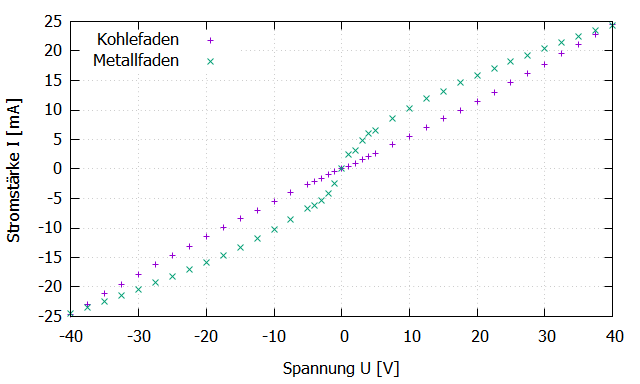
\includegraphics[scale=0.5]{V1_Kennlinien.PNG}
  \caption{Die gemessenen $U$-$I$-Kennlinien für beide Lampen}
  \label{fig:V1_Kennlinien}
\end{figure}

\begin{figure}[H]
  \centering
    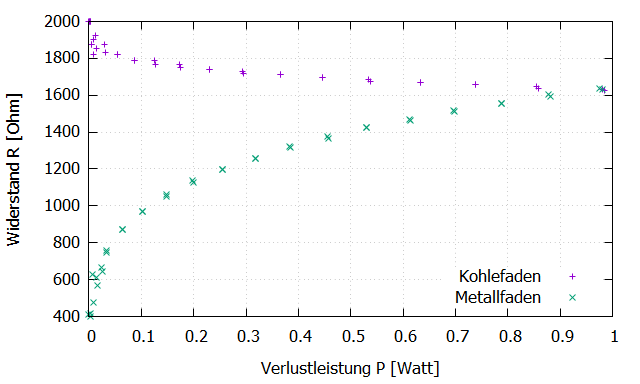
\includegraphics[scale=0.5]{V1_Leistung-Widerstand.PNG}
  \caption{Widerstand $R$ über Verlustleistung $P$ aufgetragen für beide Lampen}
  \label{fig:V1_Leistung-Widerstand}
\end{figure}
\subsection{Ergebnisdiskussion}




\pagebreak
\section{Kennlinie einer Halbleiter-Diode}
\subsection{Versuchsaufbau und Durchführung}

\begin{figure}[H]
  \centering
    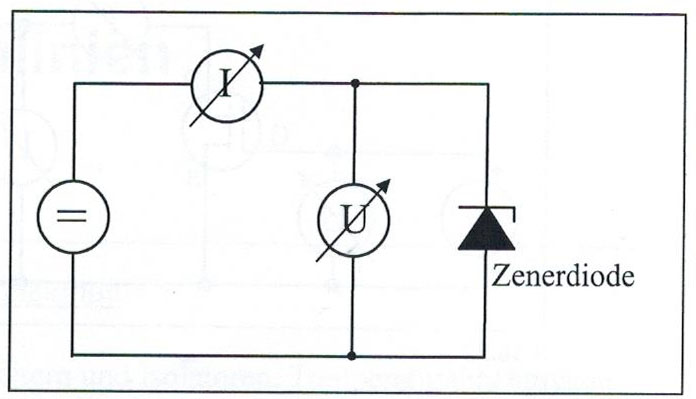
\includegraphics[scale=0.75]{Aufbau2.JPG}
  \caption{Schaltbild zur Messung an einer Halbleiter-Diode (aus der Versuchsanleitung)}
  \label{fig:Aufbau2}
\end{figure}

Der Versuchsaufbau bleibt derselbe, nur wird jetzt statt einer Lampe eine Zenerdiode eingebaut und vermessen (siehe Abbildung \ref{fig:Aufbau2}). Ziel des Versuchs ist, die Kennlinie der Diode zu erstellen. Die Spannungswerte $U$ werden so frei gewählt, dass der Verlauf der Kennlinie gut erkennbar ist, dazu wird die Stromstärke $I$ gemessen. Laut Versuchsanleitung ist eine Kennlinie wie in Abbildung \ref{fig:Kennlinie_Diode} zu erwarten. Allerdings darf der Strom nicht 200mA übersteigen, um die Diode nicht zu beschädigen.
\subsection{Messwerte und Ergebnisse}
Die Wertepaare der Kennlinie sind in Tabelle \ref{tab:Diode} aufgeführt und in Abbildung \ref{fig:V2_Kennlinie} eingetragen.

\begin{figure}[H]
  \centering
    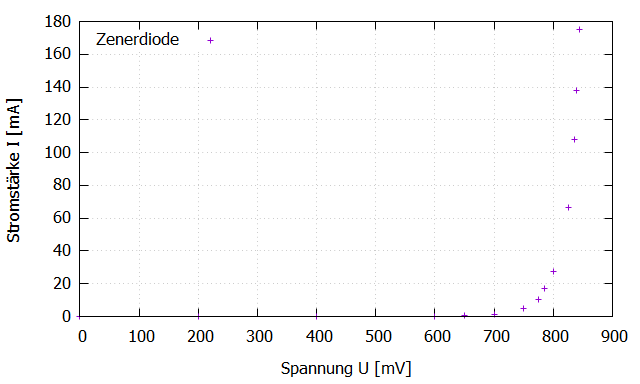
\includegraphics[scale=0.5]{V2_Kennlinie.PNG}
  \caption{Die gemessene $U$-$I$-Kennlinien der Zenerdiode}
  \label{fig:V2_Kennlinie}
\end{figure}

\begin{table}[H]
\captionof{table}{Messwerte für $I$ bei variierter Spannung $U$ für eine np-Diode.}
\begin{center}
\begin{tabular}{l|l}
U [mV]   &   I [mA] \\
\hline
-2000   &     0,0 \\
-1500   &     0,0 \\
-1000   &     0,0 \\
-500    &     0,0 \\
    0   &     0,0 \\
+200    &     0,0 \\
+400    &     0,0 \\
+600    &     0,1 \\
+650    &     0,4 \\
+700    &     1,1 \\
+750    &     5,2 \\
+775    &    10,6 \\
+785    &    16,9 \\
+800    &    27,2 \\
+825    &    66,7 \\
+835    &   107,8 \\
+840    &   138,0 \\
+845    &   175,0
\end{tabular}
\end{center}
\label{tab:Diode}
\end{table}


\subsection{Ergebnisdiskussion}

\begin{figure}[H]
  \centering
    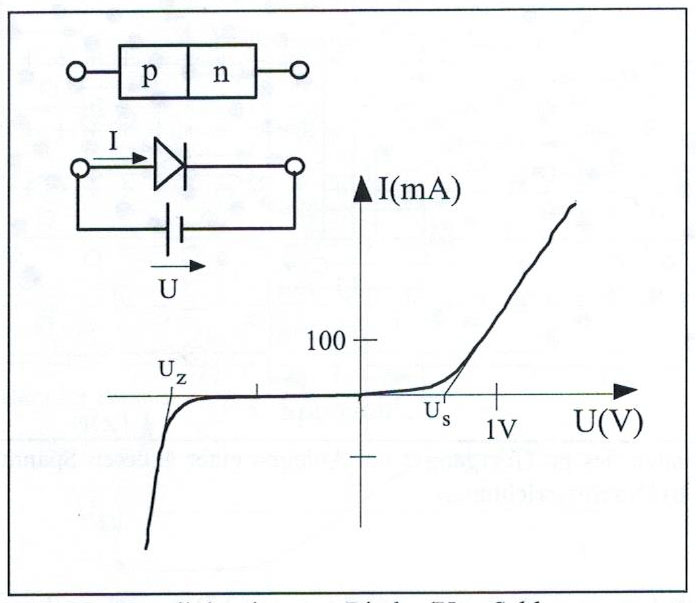
\includegraphics[scale=0.75]{Kennlinie_Diode.JPG}
  \caption{Kennlinie einer pn-Diode (aus der Versuchsanleitung)}
  \label{fig:Kennlinie_Diode}
\end{figure}




\pagebreak
\section{Halbleiter-Diode bei Wechselspannung}
\subsection{Versuchsaufbau und Durchführung}

\begin{figure}[H]
  \centering
    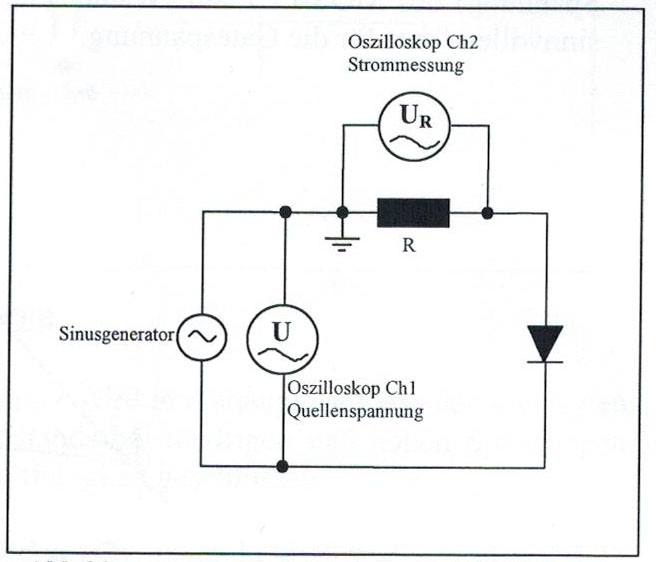
\includegraphics[scale=0.75]{Aufbau3.JPG}
  \caption{Schaltbild zur Messung mit Oszillator an einer Halbleiter-Diode (aus der Versuchsanleitung)}
  \label{fig:Aufbau3}
\end{figure}

\subsection{Messwerte und Ergebnisse}

\subsection{Ergebnisdiskussion}




\pagebreak
\section{Kennlinie eines MOS-FET}
\subsection{Versuchsaufbau und Durchführung}

\begin{figure}[H]
  \centering
    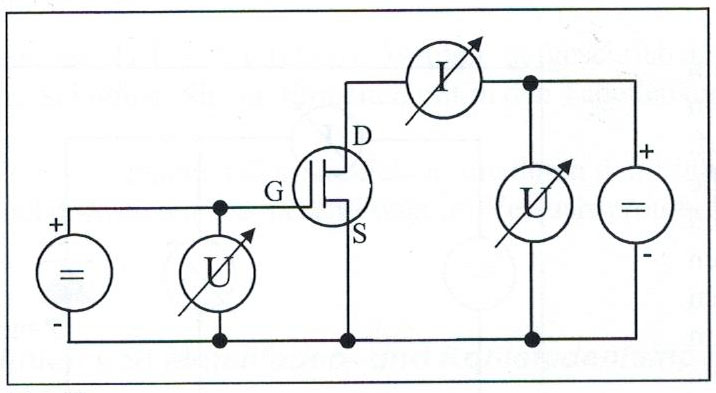
\includegraphics[scale=0.75]{Aufbau4.JPG}
  \caption{Schaltbild zur Messung an einem MOS-FET (aus der Versuchsanleitung)}
  \label{fig:Aufbau4}
\end{figure}

\subsection{Messwerte und Ergebnisse}

\subsection{Ergebnisdiskussion}

\begin{figure}[H]
  \centering
    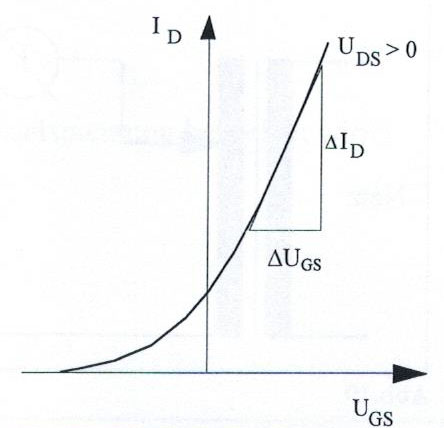
\includegraphics[scale=0.75]{Kennlinie_Gate.JPG}
  \caption{Steuerkennlinie eines selbstleitenden n-Kanal-MOS-FET (aus der Versuchsanleitung)}
  \label{fig:Kennlinie_Gate}
\end{figure}

\begin{figure}[H]
  \centering
    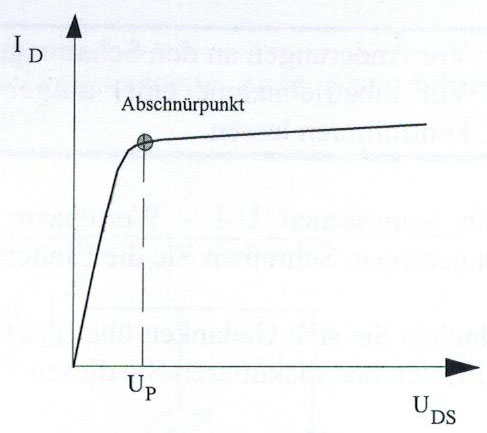
\includegraphics[scale=0.75]{Kennlinie_Drain.JPG}
  \caption{Arbeitskennlinie eines selbstleitenden n-Kanal-MOS-FET (aus der Versuchsanleitung)}
  \label{fig:Kennlinie_Drain}
\end{figure}

\end{document}
